\newtoggle{withbonus} \togglefalse{withbonus} % set true to show bonus points in grade table

% setting underlying course name (Grundlagenfach Mathematik, §-Unterricht, \ldots)
\newcommand{\mycourse}{Grundlagenfach Geografie}
% name of the class
\newcommand{\myclass}{G22s}
% set date
\newcommand{\mydate}{11. März 2025}

\title{\textbf{Prüfung: Stadtgeografie}}
\author{Cyril Wendl, Niklaus Lusser\\
	\mycourse, \myclass}
\date{\mydate}
\maketitle
\thispagestyle{headandfoot}

\begin{center}
	\fbox{\parbox{140mm}{\centering
			\begin{itemize}
				\item Dauer der Prüfung: $45$ Minuten
				      %\item \textbf{Zeige in jeder Aufgabe unbedingt Deine Schritte!}
				\item Erlaubte Hilfsmittel:
				      \begin{itemize}
					      \item Schreibzeug
					      \item Farbstifte
					      \item Leuchtstifte
				      \end{itemize}
			\end{itemize}}}
\end{center}
\vspace{10mm}

\begin{center}
	Vorname: \rule{45mm}{0.8pt}\qquad Nachname: \rule{45mm}{0.8pt}
\end{center}
\vspace{20mm}

\begin{center}
	\iftoggle{withbonus} {
		\combinedgradetable[h][questions]
	} {
		\gradetable[h][questions]
	}
\end{center}
\vspace{15mm}
\begin{center}
	Note:
	\vspace{10mm}

	\rule{8mm}{1.2pt}
\end{center}
%\thispagestyle{empty}
\clearpage

\begin{questions}
	\section*{\textcolor{Green}{Entwicklungsphasen der europäischen Stadt}}
	\question Auf folgendem Luftbild der Stadt Zürich erkennen Sie drei eingefärbte Gebiete (v.l.n.r.: orange, rot, blau). 
			\begin{figure}[H]
			\centering
			
\includegraphics[width=\linewidth, page=1,trim={4.5cm 4.7cm 1cm 1cm},clip]{"Geografie/Exam/Karte Zuerich.pdf"}
			\end{figure}
	Erläutern Sie für jedes dieser Gebiete:
	\begin{parts}
		\part[1] Name der städtebaulichen Phase:
		\fillwithlines{4cm}
		\begin{solution}
		\begin{itemize}
		\item Oranges Gebiet: Industrialisierung
		\item Rotes Gebiet: Mittelalter
		\item Blaues Gebiet: Neuzeit / Gegenwart
		\end{itemize}
		\end{solution}
		\part[1] Ungefähre zeitliche Einordnung der Städtebau-Phase:
		\fillwithlines{4cm}
		\begin{solution}
		\begin{itemize}
		\item Oranges Gebiet: 19. - 20. Jahrhundert
		\item Rotes Gebiet: 8. - 15. Jahrhundert
		\item Blaues Gebiet: 20. / 21. Jahrhundert
		\end{itemize}
		\end{solution}
		\clearpage
		\part[1] Ein räumliches Erkennungsmerkmal der städtebaulichen Periode:
		\fillwithlines{4cm}
		\begin{solution}
		\begin{itemize}
		\item Oranges Gebiet: Blockrandbebauung, Bahnhof in der Nähe
		\item Rotes Gebiet: Dichte, verwinkelte Überbauung, ``chaotischer'' / verschachtelter Grundriss
		\item Blaues Gebiet: Einfamilienhäuser, Ausrichtung entlang Strassennetz, Netz aus Haupt- und Nebenstrassen
		\end{itemize}
		\end{solution}
	\end{parts}
	
	\droptotalpoints
	
	\bonusquestion[1] Südlich vom orange eingefärbten Gebiet sehen Sie einen schmalen Wasserlauf. Wie könnte dieser entstanden sein? Achten Sie sich auf die Flussform.
	\fillwithlines{4cm}
	\begin{solution}
	Es handelt sich hierbei um einen Graben, auf dessen Grund sich früher die Zitadelle von Zürich befand (s. eckige Form der angrenzenden Gebäude). Als diese nicht mehr benötigt wurde, wurde das ehemalige Festungs-Gebiet begrünt.
	\end{solution}
	\droptotalpoints
	\vfill
	\clearpage
	\question Folgende Fotos illustrieren charakteristisch die städtebaulichen Entwicklungen der europäischen Städte von der Nachkriegszeit (ca. 1950) bis ca. im Jahr 2000.
	
	\begin{figure}[H]
	\centering
	
\includegraphics[width=\linewidth]{Private/Images/peri}
	\end{figure}
	
	\begin{parts}
	\part[2] Beschreiben Sie, was mit dem Begriff ``\textbf{Periurbanisierung}'' gemeint ist und nennen Sie die Gründe, welche dazu geführt haben.
	\fillwithlines{4cm}
		
		\begin{solution}
		Notwendige Schlüsselbegriffe, um alle Punkte zu erhalten, sind fett markiert (Synonyme möglich): 
		
		Nach dem zweiten Weltkrieg führte ein \textbf{breiter wirtschaftlicher Aufschwung} sowie technologische Entwicklungen dazu, dass eine breite Bevölkerungsschicht Zugang zu \textbf{Automobilen} und damit verbundener Mobilität erhielten. Die \textbf{Lebensqualität} in den Städten war infolge der Industrialisierung und dem Aufkommen von Fabriken teilweise schlecht, so dass ein Leben auf dem Land attraktiver schien. Mit dem Automobil konnten lange Wege schnell zurückgelegt werden, so dass viele Menschen ein schönes Einfamilienhaus auf dem Land einer kleinen, engen Stadtwohnung bevorzugten. Mit der Suburbanisierung ist also eine \textbf{Verlagerung von städtischen und stadtnahen (suburbanen) Gebieten in entlegenere, ländlichere (periurbanere) Gebiete} gemeint.
			\end{solution}
			\part[2] Erklären Sie den Begriff ``\textbf{Reurbanisierung}'', indem Sie 2 Gründe nennen, welche zur Reurbanisierung geführt haben, sowie 2 Massnahmen, um die Reurbanisierung voranzutreiben.
			\fillwithlines{4cm} 
			\begin{solution}
			\textbf{Mehrere Gründe möglich}:
			\begin{itemize}
			\item Sinkende Steuereinnahmen der Städte
			\item Tägliche zeitliche Einbussen durch Pendeln
			\item Mehrausgaben für Autobesitz
			\item Leben auf dem Land für gewisse Bevölkerungsschichten (Nachwuchs der Babyboomer) weniger attraktiv
			\end{itemize}
			
			\textbf{Massnahmen}:
			\begin{itemize}
			\item Finanzielle Anreize (günstiger Wohnraum): Grosswohnsiedlungen, Verdichtung gegen innen
			\item Förderung von ÖV innerhalb und zwischen den Städten
			\end{itemize}
			\end{solution}
	\end{parts}	
	
	\droptotalpoints
	\clearpage
	
	\section*{\textcolor{Green}{Weltweite Städte}}
	\question[2\half] Auf folgendem Luftbild von Google Earth erkennen Sie die Stadt Los Angeles in den USA. Nennen und erläutern Sie mindestens 5 zentrale Aspekte nordamerikanischer Städte, indem Sie diese Aspekte auf der Karte einzeichnen, benennen und erklären, was damit gemeint ist.
	\begin{figure}[H]
	\centering
	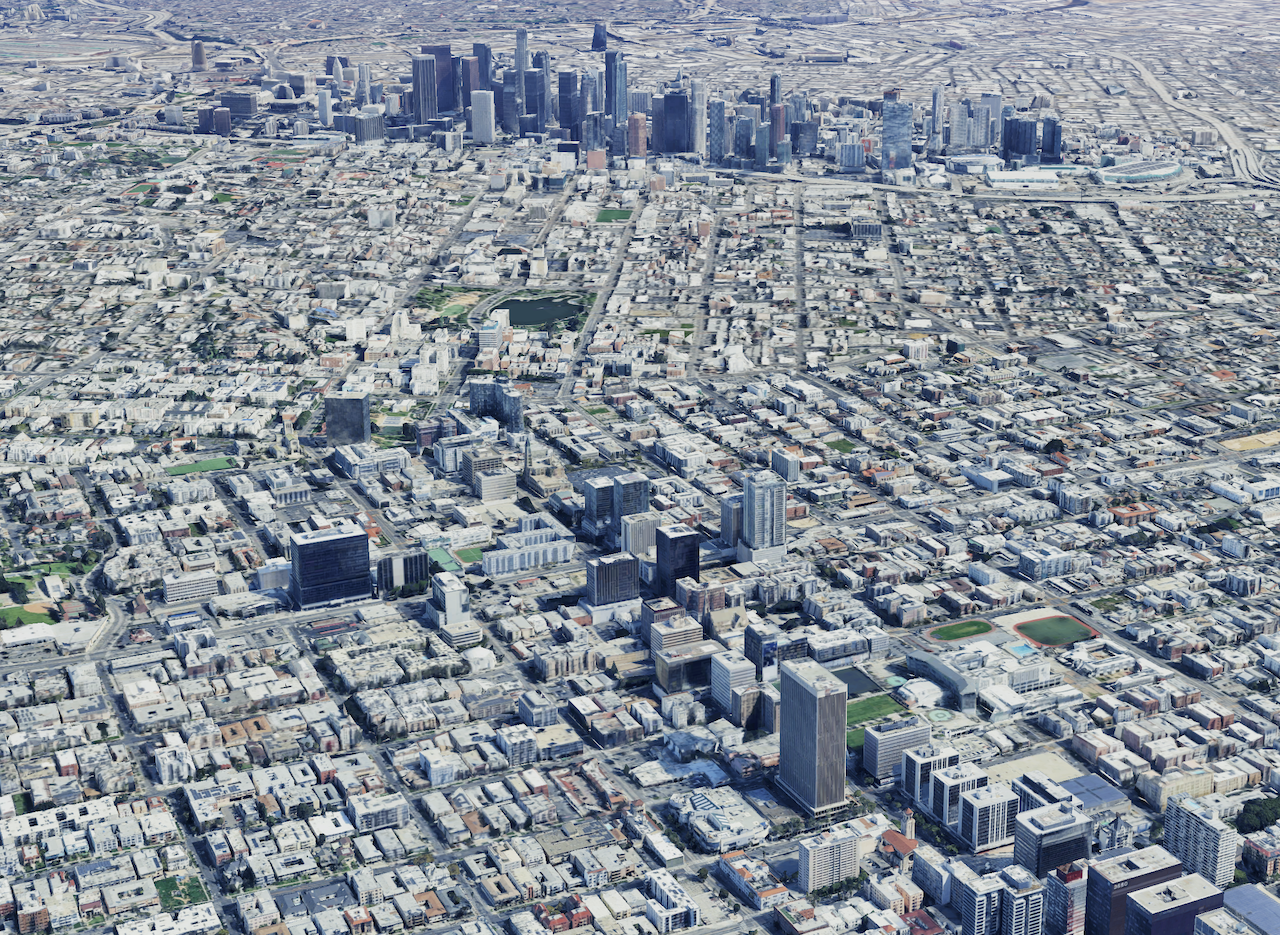
\includegraphics[width=\linewidth]{Geografie/Exam/LA}
	\end{figure}
	\begin{solution}
		\begin{figure}[H]
		\centering
		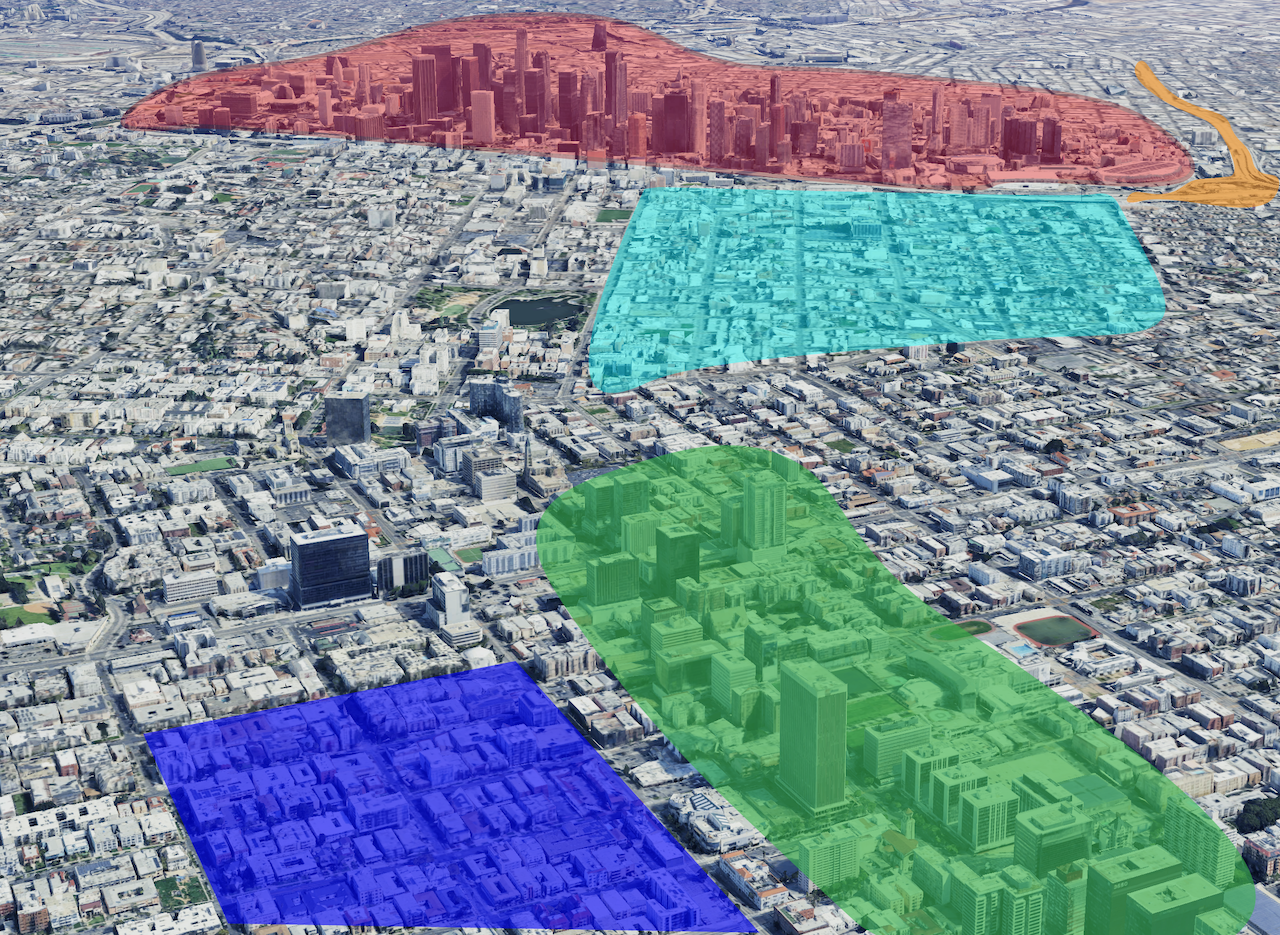
\includegraphics[width=0.7\linewidth]{Geografie/Exam/LA_sol}
		\end{figure}
		0.5 Punkte pro richtige Antwort:
			\begin{itemize}
			\item Rot: CBD, zentrales Hochhausgebiet, meist bestehend aus vorwiegend Geschäftsgebäuden
			\item Orange: Autoinfrastruktur (auch andernorts sichtbar), welche benötigt wird, um in die vielfach weit entlegenen Wohngebiete zu gelangen
			\item Hellblau: Übergangsbereich, häufig mit sozialer Segregation (afroamerikanische Bevölkerung), günstigen Wohnräumen und Parkplätzen, teilweise saniert
			\item Dunkelblau: Schachbrettmuster, zeigt den planmässigen Aufbau amerikanischer Städte
			\item Grün: Edge City, eine ``Mini-Stadt'' mit einem kleinen ``Mini-CBD'', welche in der Nähe der suburbanen Wohngebiete entstanden ist.
			\end{itemize}
	\end{solution}	
	\fillwithlines{\stretch{1}}
	\droptotalpoints
	\clearpage
	\question
	Betrachten Sie folgendes Bild:
	\begin{figure}[H]
	\centering
	\includegraphics[width=.6\linewidth]{"Private/Images/Orient-Stadt/strasse-rabat"}
	\end{figure}
	\begin{parts}
	\part[1] Nennen Sie einen Begriff, um das auf dem Bild Dargestellte am treffendsten zu bezeichnen.
	\fillwithlines{1cm}
	\begin{solution}
	Souk oder Markt
	\end{solution}
	\part[1] In welchem (grösseren) Stadtteil befindet sich dieses Bild?
	\fillwithlines{1cm}
	\begin{solution}
	Medina oder Altstadt
	\end{solution}
	\part[1] In welchem Stadt-Modell ist das Bild zu verorten?
	\fillwithlines{1cm}
	
	\begin{solution}
	Die orientalische Stadt
	\end{solution}
	\end{parts}
	\droptotalpoints
	
	\clearpage
	\section*{\textcolor{Green}{Nachhaltige Stadtmodelle}}
	\question[4\half] Vervollständigen Sie folgende Tabelle, indem Sie für jedes Stadt-Modell in 1-2 ganzen Sätzen erklären, wann es entstanden ist, aus welchen Gründen und welche Haupt-Ziele damit verfolgt wurden.
	
	\begin{table}[H]
	\centering
	\begin{tabular}{p{.15\textwidth}|p{.25\textwidth}|p{.25\textwidth}|p{.25\textwidth}}
	\textbf{Stadt-Modell} & \textbf{Ungefährer \newline Entstehungszeitraum} & \textbf{Gründe, die zur \newline Entstehung führten} & \textbf{Haupt-Ziele \newline des Modells} \\\midrule
	\textbf{Gartenstadt} &&&\\[90pt]\midrule
	\textbf{Die \newline gegliederte \newline Stadt} &&&\\[90pt]\midrule
	\textbf{Die Stadt der kurzen Wege} &&& \\[90pt]
	\end{tabular}
	\end{table}
	\begin{solution}
	.5 Punkte pro richtige Antwort (pro richtiges Feld):
		\begin{table}[H]
		\small
		\centering
		\begin{tabular}{p{.15\textwidth}|p{.25\textwidth}|p{.25\textwidth}|p{.25\textwidth}}
		\textbf{Stadt-Modell} & \textbf{Ungefährer \newline Entstehungszeitraum} & \textbf{Gründe, die zur \newline Entstehung führten} & \textbf{Haupt-Ziele \newline des Modells} \\\midrule
		\textbf{Gartenstadt} &Anfang 20. Jahrhundert &Industrialisierung, verschmutzte Städte& Mehr Grünraum schaffen auf kompaktem Raum, Naherholungsgebiete\\[60pt]\midrule
		\textbf{Die\newline gegliederte\newline Stadt} &Mitte 20. Jahrhundert&Zersiederlung der Landschaft stoppen, funktionale Gliederung der Stadt& Hochhäuser bauen und Grunddaseinsfunktionen trennen.\\[60pt]\midrule
		\textbf{Die\newline Stadt\newline der\newline kurzen\newline Wege} &Ende 20. Jahrhundert&Auto-zentrierte Stadt führt zu schlechter Lebensqualität, Pendlerwege reduzieren& Alle wichtigen Grunddaseinsfunktionen in $<$15 Minuten erreichbar machen. \\[60pt]
		\end{tabular}
		
		\end{table}
	\end{solution}
	\droptotalpoints
	\clearpage
	\bonusquestion[2] Würde die Erstellung eines Superblocks in Sursee ebenfalls Sinn ergeben? Wenn ja, weshalb? Wenn nein, weshalb? Welche Gründe sprechen in Sursee stärker für oder gegen die Erstellung von Superblocks gegenüber anderen Städten?
	
	\begin{solution}
	Gründe, welche allgemein und unabhängig vom Standort für Superblocks sprechen, sind starkes Verkehrsaufkommen bei hoher Bevölkerungsdichte. Beides scheint in Sursee weniger gegeben zu sein als in grösseren Städten, insofern scheinen Superblocks in Sursee weniger notwendig als andernorts. Die Nachteilseite wäre zudem teilweise grösser: Städte wie Sursee sind stärker auf das Auto (und Parkplätze) angewiesen als kleinere Städte, weshalb kleine Betriebe und Läden unter der Massnahme leiden könnten. Die Attraktivität von Wohnungen in autofreien Zonen könnte geschwächt statt gestärkt werden. Auf der Kehrseite scheinen Bedenken hinsichtlich Sicherheit und Gentrifizierung vermutlich reduziert.
	\end{solution}
	\fillwithlines{4cm}
	\droppoints
\end{questions}

\clearpage
(leere Seite für Notizen)
\clearpage
(leere Seite für Notizen)
